\documentclass{article}

% Language setting
% Replace `english' with e.g. `spanish' to change the document language
\usepackage[english]{babel}

% Set page size and margins
% Replace `letterpaper' with `a4paper' for UK/EU standard size
\usepackage[a4paper,top=2cm,bottom=2cm,left=3cm,right=3cm,marginparwidth=1.75cm]{geometry}

% Useful packages
\usepackage{amsmath}
\usepackage{graphicx}
\usepackage[colorlinks=true, allcolors=blue]{hyperref}
\usepackage{xcolor}
\usepackage{listings}
\usepackage{multicol}
\colorlet{mygray}{black!30}
\colorlet{mygreen}{green!60!blue}
\colorlet{mymauve}{red!60!blue}



\lstdefinelanguage{makefile}{
otherkeywords={.SUFFIXES},
morekeywords={SUFFIX, CPP_,},
moredelim=[is][\color{mbleu}]{/*}{*/},
style=global,%
morecomment=[l][commentstyle]{\#},%
emphstyle={\color{vimvert}},%
moredelim=[s][\color{vimvert}]{\$(}{)}%
}

\lstdefinelanguage{cpp}{
  backgroundcolor=\color{gray!10},  
  basicstyle=\ttfamily,
  columns=fullflexible,
  breakatwhitespace=false,      
  breaklines=true,                
  captionpos=b,                    
  commentstyle=\color{mygreen}, 
  extendedchars=true,              
  frame=single,                   
  keepspaces=true,             
  keywordstyle=\color{blue},      
  language=c++,                 
  numbers=none,                
  numbersep=5pt,                   
  numberstyle=\tiny\color{blue}, 
  rulecolor=\color{mygray},        
  showspaces=false,
  showstringspaces=false,
  showtabs=false,                 
  stepnumber=5,                  
  stringstyle=\color{mymauve},    
  tabsize=3,                                     
  title=\lstname 
}
\lstset{language=cpp}
\lstnewenvironment{code}[2][]{%
  \lstset{%
    numbers = left,
    title   = #2,
    #1,
  }%
}{}

\title{Embedded Systems Programming \\ Assignment 4.1 \\ \large Embedded Linux}
\author{Steinarr Hrafn Höskuldsson}

\usepackage{fancyhdr}
\fancypagestyle{firststyle}
{
   \fancyhf{}
   \fancyhead[L]{Embedded Systems Programming}
   
   \renewcommand{\headrulewidth}{0pt} % removes horizontal header line
}

\newcommand{\mycomment}[1]{}
\begin{document}
\pagestyle{firststyle}
{\let\newpage\relax\maketitle}

\mycomment{
\begin{figure}[h]
    \centering
    \includegraphics[width=0.75\textwidth]{LAB3/Basic1.png}
    \caption{"Switch test" Breadboard set up}
    \label{fig:Switch_test}
\end{figure}

\lstinputlisting[caption=main.cpp in Part 3]{Assignment3_1StateBehaviour/src/main_prt3.cpp}

}

\section*{Part 1}
The kernel headers were installed without issues. The \verb!hello! kernel example from L4.4 was used and the Makefile from L4.3 was used to compile it.

\begin{lstlisting}[caption={The output of modinfo}]
pi@raspberrypi:~/EmbeddedAssignments/Assignment4_2LinuxKernelModule $ sudo modinfo hello.ko
filename:       /home/pi/EmbeddedAssignments/Assignment4_2LinuxKernelModule/hello.ko
version:        0.1
description:    A simple Linux LKM that accepts characters (bytes) from the user.
author:         Steinarr Hrafn
license:        GPL
srcversion:     61AB8CCEEFA7BB47532F8F3
depends:        
name:           hello
vermagic:       5.15.61-v7+ SMP mod_unload modversions ARMv7 p2v8 
parm:           name:The name to display in /var/log/kern.log (charp)
\end{lstlisting}

The kernel module was loaded and unloaded while the kernel output log was being monitored. 
\begin{figure}[h]
    \centering
    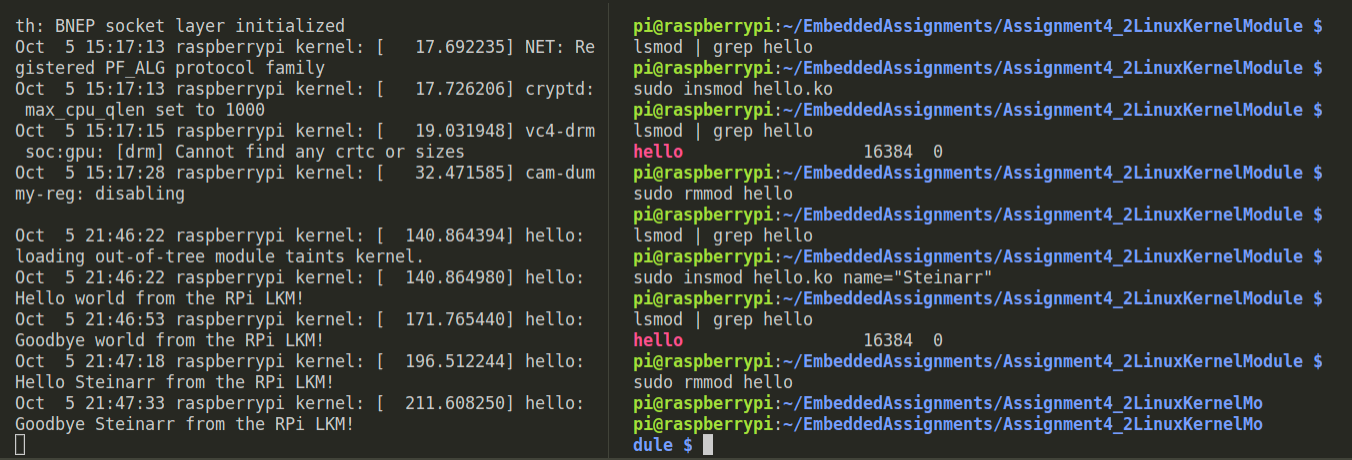
\includegraphics[width=\textwidth]{Assignment4_2LinuxKernelModule/part1_kernel_loading.png}
    \caption{Screenshot of the terminals used to test the loading and unloading of the hello kernel module.}
    \label{fig:kernel_loading}
\end{figure}

\newpage
\section*{Part 2}


\section*{Part 3}
The \verb!increment! and \verb!decrement! implementations were copied to \verb!increment_fifo! and \verb!decrement_fifo! and modified so that increment adds an integer to the queue and \verb!decrement! gets an integer, the implementations can be seen in Appendix \ref{appendix:fifoments}. The \verb!Fifo! implementation was modified so that the inner workings of it were protected with the MutEx.
\lstinputlisting[caption=Thread safe implementation of a First-in-First-out Queue. ]{Assignment4_1EmbeddedLinux/src/fifo3.cpp}
\verb!main_fifo.cpp! was written to start the \verb!increment! and \verb!decrement! threads. 

\lstinputlisting[caption=src/main\_fifo.cpp]{Assignment4_1EmbeddedLinux/src/main_fifo.cpp}
The Makefile was edited to compile \verb!main_fifo!
\lstinputlisting[language=makefile, caption=The Makefile used to compile main\_fifo.cpp]{Assignment4_1EmbeddedLinux/Makefile}
\section*{Appendix}
\appendix
\section{Output from Part 1}
\begin{lstlisting}[caption={src/hello.cpp, writes "Hello" to stdout}]
pi@raspberrypi:~/EmbeddedAssignments/Assignment4_2LinuxKernelModule $ lsmod | grep hello
pi@raspberrypi:~/EmbeddedAssignments/Assignment4_2LinuxKernelModule $ sudo insmod hello.ko
pi@raspberrypi:~/EmbeddedAssignments/Assignment4_2LinuxKernelModule $ lsmod | grep hello
hello                  16384  0
pi@raspberrypi:~/EmbeddedAssignments/Assignment4_2LinuxKernelModule $ sudo rmmod hello
pi@raspberrypi:~/EmbeddedAssignments/Assignment4_2LinuxKernelModule $ lsmod | grep hello
pi@raspberrypi:~/EmbeddedAssignments/Assignment4_2LinuxKernelModule $ sudo insmod hello.ko name="Steinarr"
pi@raspberrypi:~/EmbeddedAssignments/Assignment4_2LinuxKernelModule $ lsmod | grep hello
hello                  16384  0
pi@raspberrypi:~/EmbeddedAssignments/Assignment4_2LinuxKernelModule $ sudo rmmod hello
\end{lstlisting}

\begin{lstlisting}

Oct  5 21:46:22 raspberrypi kernel: [  140.864394] hello: loading out-of-tree module taints kernel.
Oct  5 21:46:22 raspberrypi kernel: [  140.864980] hello: Hello world from the RPi LKM!
Oct  5 21:46:53 raspberrypi kernel: [  171.765440] hello: Goodbye world from the RPi LKM!
Oct  5 21:47:18 raspberrypi kernel: [  196.512244] hello: Hello Steinarr from the RPi LKM!
\end{lstlisting}
\end{document}

